\chapter{Continuous Random Variables}

So far, we have studied discrete random variables and we have explored their properties.
Discrete random variables are quite useful in many contexts, yet they form only a small subset of the collection of random variables pertinent to applied probability and engineering.
In this chapter, we consider random variables that range over a continuum of possible values; that is, random variables that can take on an uncountable set of values.

Continuous random variables are powerful mathematical abstractions that allow engineers to pose and solve important problems.
Many of these problems are difficult to address using discrete models.
While this extra flexibility is useful and desirable, it comes at a certain cost.
A continuous random variable cannot be characterized by a probability mass function.
This predicament emerges from the limitations of the third axiom of probability laws, which only applies to countable collections of disjoint events.

Below, we provide a definition for continuous random variables.
Furthermore, we extend and apply the concepts and methods initially developed for discrete random variables to the class of continuous random variables.
In particular, we develop a continuous counterpart to the probability mass function.


\section{Cumulative Distribution Functions}

We begin our exposition of continuous random variables by introducing a general concept which can be employed to bridge our understanding of discrete and continuous random variables.
Recall that a \emph{random variable} is a real-valued function acting on the outcomes of an experiment. \index{Random variable}
In particular, given a sample space, random variable $X$ is a function from $\Omega$ to $\RealNumbers$.
The \emph{cumulative distribution function (CDF)} of $X$ is defined point-wise as the probability of the event $\{X \leq x \}$, \index{Cumulative distribution function}
\begin{equation*}
F_X (x) = \Pr ( \{ X \leq x \} ) = \Pr (X \leq x).
\end{equation*}
In terms of the underlying sample space, $F_X (x)$ denotes the probability of the set of all outcomes in $\Omega$ for which the value of $X$ is less than or equal to $x$,
\begin{equation*}
F_X (x) = \Pr \left( X^{-1} ( (- \infty, x]) \right)
= \Pr (\{ \omega \in \Omega | X(\omega) \leq x \}).
\end{equation*}
In essence, the CDF is a convenient way to specify the probability of all events of the form $\{ X \in (-\infty, x] \}$.

The CDF of random variable $X$ exists for any well-behaved function $X : \Omega \mapsto \RealNumbers$.
Moreover, since the realization of $X$ is a real number, we have
\begin{gather*}
\lim_{x \downarrow - \infty} F_X (x) = 0 \\
\lim_{x \uparrow \infty} F_X (x) = 1.
\end{gather*}
Suppose $x_1 < x_2$, then we can write $\{ X \leq x_2 \}$ as the union of the two disjoint sets $\{ X \leq x_1 \}$ and $\{ x_1 < X \leq x_2 \}$.
It follows that
\begin{equation} \label{equation:NonDecreasingCDF}
\begin{split}
F_X (x_2) &= \Pr (X \leq x_2) \\
&= \Pr (X \leq x_1) + \Pr (x_1 < X \leq x_2) \\
&\geq \Pr (X \leq x_1) = F_X (x_1).
\end{split}
\end{equation}
In other words, a CDF is always a non-decreasing function.
Finally, we note from \eqref{equation:NonDecreasingCDF} that the probability of $X$ falling in the interval $(x_1, x_2]$ is
\begin{equation} \label{equation:IntervalCDF}
\Pr (x_1 < X \leq x_2) = F_X (x_2) - F_X (x_1).
\end{equation}


\subsection{Discrete Random Variables}

If $X$ is a discrete random variable, then the CDF of $X$ is given by
\begin{equation*}
F_X (x) = \sum_{u \in X(\Omega) \cap (-\infty, x]} p_X (u),
\end{equation*}
and its PMF can be computed using the formula
\begin{equation*}
p_X (x) = \Pr (X \leq x) - \Pr (X < x) = F_X (x) - \lim_{u \uparrow x} F_X (u).
\end{equation*}
Fortunately, this formula is simpler when the random variable $X$ only takes integer values, as seen in the example below.

\begin{figure}[ht]
\begin{center}
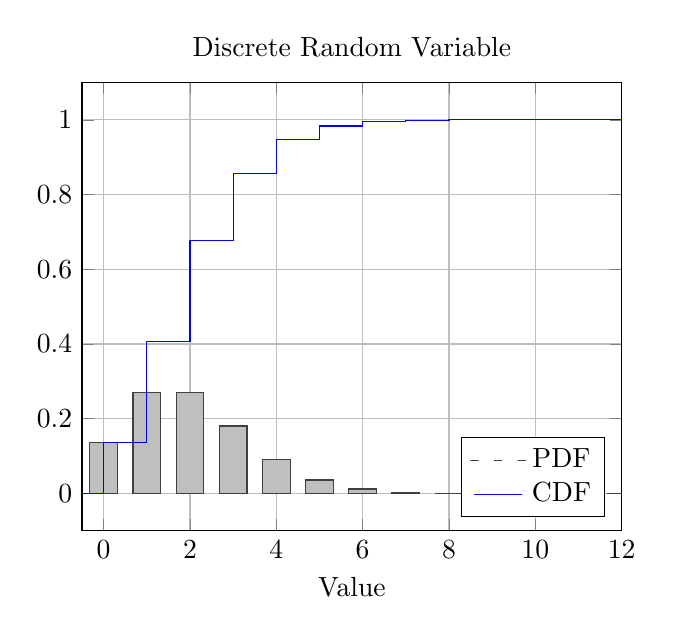
\begin{tikzpicture}
\begin{axis}[
    title={Discrete Random Variable},
    xlabel={Value},
	xmajorgrids,
	xmin=-0.5, xmax=12,
	ymajorgrids,
	legend pos=south east]
\addplot[ybar,darkgray,fill=lightgray]
    coordinates
    {(0, 0.135335283) (1, 0.270670566) (2, 0.270670566) (3, 0.180447044)
    (4, 0.090223522) (5, 0.036089409) (6, 0.012029803) (7, 0.003437087)
    (8, 0.000859272) (9, 0.000190949) (10, 0.0000381899) (11, 0.00000694361)
	(12, 0.00000115727)};
\addlegendentry{PDF}
\addplot[blue] coordinates
	{(-0.5, 0) (0,0)
	(0, 0.135335283) (1, 0.135335283)
	(1,0.406005850) (2,0.406005850)
	(2,0.676676416) (3,0.676676416)
	(3,0.857123460) (4,0.857123460)
	(4,0.947346983) (5,0.947346983)
	(5,0.983436392) (6,0.983436392)
	(6,0.995466194) (7,0.995466194)
	(7,0.998903281) (8,0.998903281)
	(8,0.999762553) (9,0.999762553)
	(9,0.999953502) (10,0.999953502)
	(10,0.999991692) (11,0.999991692)
	(11, 0.999998635) (12, 0.999998635)};
\addlegendentry{CDF}
\end{axis}
\end{tikzpicture}
\end{center}
\caption{This figure shows the PMF of a discrete random variable, along with the corresponding CDF.
The values of the PMF are depicted by the height of the rectangles; their cumulative sums lead to the values of the CDF.}
\end{figure}

\begin{example}
Let $X$ be a geometric random variable with parameter $p$,
\begin{equation*}
p_X (k) = (1 - p)^{k-1} p \quad k = 1, 2, \ldots 
\end{equation*}
For $x > 0$, the CDF of $X$ is given by
\begin{equation*}
F_X (x) = \sum_{k = 1}^{\lfloor x \rfloor} (1 - p)^{k-1} p
= 1 - (1 - p)^{\lfloor x \rfloor} ,
\end{equation*}
where $\lfloor \cdot \rfloor$ denotes the standard floor function.
For integer $k \geq 1$, the PMF of geometric random variable $X$ can be recovered from the CDF as follows,
\begin{equation*}
\begin{split}
p_X (k) &= F_X (x) - \lim_{u \uparrow x} F_X (u) = F_X (k) - F_X (k-1) \\
&= \left( 1 - (1-p)^k \right) - \left( 1 - (1-p)^{k-1} \right) \\
%&= (1 - p)^{k-1} - (1-p) (1-p)^{k-1} \\
&= (1 - p)^{k-1} p .
\end{split}
\end{equation*}
\end{example}


\subsection{Continuous Random Variables}

Having introduced the general notion of a CDF, we can safely provide a more precise definition for continuous random variables.
Let $X$ be a random variable with CDF $F_X (\cdot)$, then $X$ is said to be a \emph{continuous random variable} if $F_X (\cdot)$ is continuous and differentiable. \index{Continuous random variable}

\begin{example}
Suppose that $X$ is a random variable with CDF given by
\begin{equation*}
F_X(x) = \begin{cases} 1 - e^{-x}, & x \geq 0 \\
0, & x < 0 . \end{cases}
\end{equation*}
This cumulative distribution function is differentiable with
\begin{equation*}
\frac{dF_X}{dx}(x)
= \begin{cases} e^{-x}, & x > 0 \\
0, & x < 0 \end{cases}
\end{equation*}
and therefore $X$ is a continuous random variable.
\end{example}

\begin{figure}[ht]
\begin{center}
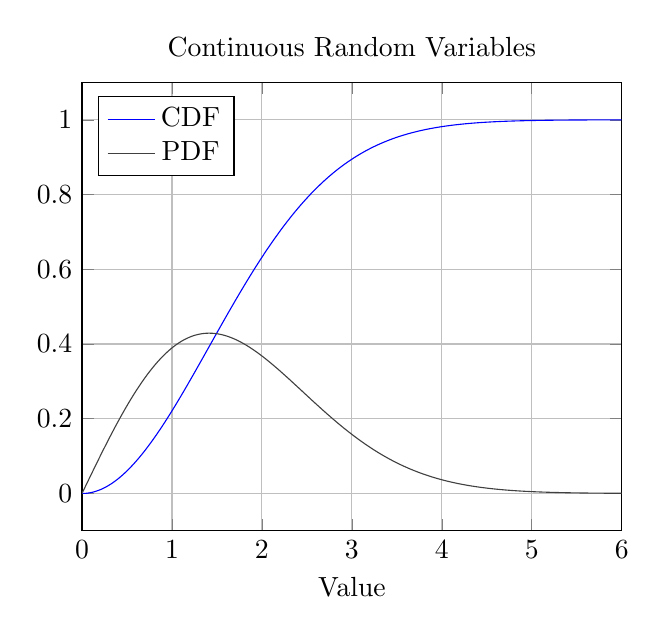
\begin{tikzpicture}
\begin{axis}[
	title={Continuous Random Variables},
	xlabel={Value},
	xmin=0, xmax=6,
	xmajorgrids,
	ymajorgrids,
	legend pos=north west]
\addplot[blue,domain=0:6,samples=201]
	{1 - exp(-0.25*(x^2))};
\addlegendentry{CDF}

\addplot[darkgray,domain=0:6,samples=201]
	{0.5*x*exp(-0.25*(x^2))};
\addlegendentry{PDF}
\end{axis}
\end{tikzpicture}
\end{center}
\caption{The CDF of a continuous random variable is differentiable.
This figure provides one example of a continuous random variable.
Both, the CDF $F_X(\cdot)$ and its derivative $f_X(\cdot)$ (PDF) are displayed.}
\end{figure}


\subsection{Mixed Random Variables*}

Generally speaking, the CDF of a discrete random variable is a discontinuous staircase-like function, whereas the CDF of a continuous random variable is continuous and differentiable almost everywhere.
There exist random variables for which neither situation applies.
Such random variables are sometimes called \emph{mixed random variables}. \index{Mixed random variable}
Our exposition of mixed random variables in this document is very limited.
Still, we emphasize that a good understanding of discrete and continuous random variables is instrumental in understanding and solving problems including mixed random variables.

\begin{figure}[ht]
\begin{center}
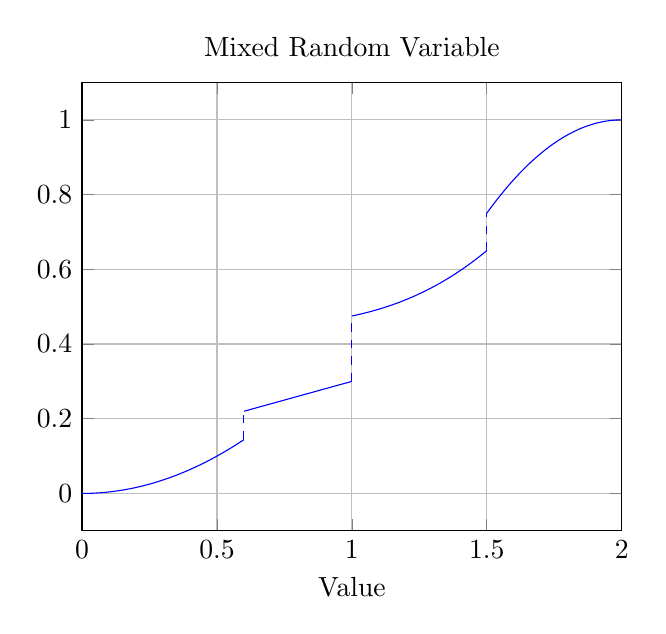
\begin{tikzpicture}
\begin{axis}[
    title={Mixed Random Variable},
    xlabel={Value},
	xmin=0, xmax=2,
	xmajorgrids,
	ymajorgrids,
    legend pos=north west]
\addplot[blue,domain=0:0.6,samples=61]
	{0.4*(x^2)};
\addplot[blue,domain=0.6:1,samples=41]
	{0.1 + 0.2*x};
\addplot[blue,domain=1:1.5,samples=51]
	{0.25 + 0.2*(1 + (x-0.5)^3)};
\addplot[blue,domain=1.5:2,samples=51]
	{1 - (x-2)^2};
\addplot[blue,dashed] coordinates {
	(0.6,0.144) (0.6,0.22)

	(1,0.3) (1,0.475)

	(1.5,0.65) (1.5,0.75)};
\end{axis}
\end{tikzpicture}
\end{center}
\caption{This figure shows the CDF of a mixed random variable.
In general, mixed random variables do not have a PMF nor a PDF.
Their CDF may be composed of a mixture of differentiable intervals and discontinuous jumps.}
\end{figure}


\section{Probability Density Functions}

As mentioned above, the CDF of continuous random variable $X$ is a differentiable function.
The derivative of $F_X (\cdot)$ is called the \emph{probability density function (PDF)} of $X$, and it is denoted by $f_X(\cdot)$. \index{Probability density function (PDF)}
If $X$ is a random variable with PDF $f_X (\cdot)$ then, by the fundamental theorem of calculus, we have
\begin{equation*}
F_X (x) = \int_{- \infty}^x f_X (u) du .
\end{equation*}
Equivalently, we can write
\begin{equation*}
f_X (x) = \frac{d F_X}{dx} (x) .
\end{equation*}
Note that PDFs are only defined for continuous random variables.
This is somewhat restrictive.
Nevertheless, the PDF can be a very powerful tool to derive properties of continuous random variables, which may otherwise be difficult to compute.

For $x_1 < x_2$, we can combine the definition of $f_X(\cdot)$ and \eqref{equation:IntervalCDF} to obtain
\begin{equation*}
\Pr (x_1 < X \leq x_2) = \int_{x_1}^{x_2} f_X (u) du .
\end{equation*}
Furthermore, it is easily seen that for any continuous random variable
\begin{equation*}
\begin{split}
\Pr (X = x_2) &= \lim_{x_1 \uparrow x_2} \Pr (x_1 < X \leq x_2)
= \lim_{x_1 \uparrow x_2} \int_{x_1}^{x_2} f_X (u) du \\
&= \int_{x_2}^{x_2} f_X (u) du = 0.
\end{split}
\end{equation*}
In other words, if $X$ is a continuous random variable, then $\Pr (X = x) = 0$ for any real number $x$.
An immediate corollary of this fact is
\begin{equation*}
\begin{split}
&\Pr (x_1 < X < x_2)
= \Pr (x_1 \leq X < x_2) \\
&= \Pr (x_1 < X \leq x_2)
= \Pr (x_1 \leq X \leq x_2) ;
\end{split}
\end{equation*}
the inclusion or exclusion of endpoints in an interval does not affect the probability of the corresponding interval when $X$ is a continuous random variable.

We can derive properties for the PDF of continuous random variable $X$ based on the axioms of probability laws.
First, the probability that $X$ is a real number is given by
\begin{equation*}
\Pr (-\infty < X < \infty) = \int_{-\infty}^{\infty} f_X (u) du = 1.
\end{equation*}
Thus, $f_X (x)$ must integrate to one.
Also, because the probabilities of events are nonnegative, we must have $f_X (x) \geq 0$ everywhere.
Finally, given an admissible set $S$, the probability that $X \in S$ can be expressed through an integral,
\begin{equation*}
\Pr (X \in S) = \int_S f_X (u) du .
\end{equation*}
Admissible events of the form $\{ X \in S \}$ are sets for which we know how to carry this integral.


\section{Expectation Revisited}

The definition of an expectation associated with a continuous random variable is very similar to its discrete counterpart;
the weighted sum is simply replaced by a weighted integral.
For a continuous random variable $X$ with PDF $f_X(\cdot)$, the \emph{expectation} of $g(X)$ is defined by \index{Expectation}
\begin{equation*}
\Expect [g(X)]
= \int_{\RealNumbers} g(u) f_X (u) du .
\end{equation*}
In particular, the \emph{mean} of $X$ is equal to \index{Mean}
\begin{equation*}
\Expect [X]
= \int_{\RealNumbers} u f_X (u) du
\end{equation*}
and its \emph{variance} becomes \index{Variance}
\begin{equation*}
\Var [X] = \Expect \left[ (X - \Expect[X])^2 \right]
= \int_{\RealNumbers} (u - \Expect[X])^2 f_X (u) du .
\end{equation*}
As before, the variance of random variable $X$ can also be computed using $\Var [X] = \Expect \left[ X^2 \right] - \left( \Expect [X] \right)^2$.



For nonnegative random variable $X$, an alternative way to compute $\Expect [X]$ is described in Proposition~\ref{proposition:MeanAlternative}. \index{Expectation}

\begin{proposition} \label{proposition:MeanAlternative}
Suppose that $X$ is a nonnegative random variable with finite mean, then
\begin{equation*}
\Expect [X] = \int_0^{\infty} \Pr (X > x) dx .
\end{equation*}
\end{proposition}
\begin{proof}
We offer a proof for the special case where $X$ is a continuous random variable, although the result remains true in general,
\begin{equation*}
\begin{split}
\int_0^{\infty} \Pr (X > x) dx
&= \int_0^{\infty} \int_x^{\infty} f_X(u) du dx \\
&= \int_0^{\infty} \int_0^{u} f_X(u) dx du \\
&= \int_0^{\infty} u f_X(u) du
= \Expect [X] .
\end{split}
\end{equation*}
Interchanging the order of integration is justified because $X$ is assumed to have finite mean.
\end{proof}

\begin{example}
A player throws darts at a circular target hung on a wall.
The dartboard has unit radius, and the position of every dart is distributed uniformly over the target.
We wish to compute the expected distance from each dart to the center of the dartboard.

Let $R$ denote the distance from a dart to the center of the target.
For $0 \leq r \leq 1$, the probability that $R$ exceeds $r$ is given by
\begin{equation*}
\Pr (R > r) = 1 - \Pr (R \leq r) = 1 - \frac{\pi r^2}{\pi} = 1 - r^2 .
\end{equation*}
Then, by Proposition~\ref{proposition:MeanAlternative}, the expected value of $R$ is equal to
\begin{equation*}
\Expect [R] = \int_0^1 \left( 1 - r^2 \right) dr
= \left.  \left( r - \frac{r^3}{3} \right) \right|_0^1
= 1 - \frac{1}{3} = \frac{2}{3} .
\end{equation*}
Notice how we were able to compute the answer without deriving an explicit expression for $f_R (\cdot)$.
\end{example}


\section{Important Distributions}

Good intuition about continuous random variables can be developed by looking at examples.
In this section, we introduce important random variables and their distributions.
These random variables find widespread application in various fields of engineering.


\subsection{The Uniform Distribution}

A (continuous) \emph{uniform random variable} is such that all intervals of a same length contained within its support are equally probable. \index{Uniform random variable (continuous)}
The PDF of a uniform random variable is defined by two parameters, $a$ and $b$, which represent the minimum and maximum values of its support, respectively.
The PDF $f_X(\cdot)$ is given by
\begin{equation*}
f_X(x) = \begin{cases} \frac{1}{b-a}, & x \in [a, b] \\
0, & \text{otherwise}. \end{cases}
\end{equation*}
The associated cumulative distribution function becomes
\begin{equation*}
F_X(x) = \begin{cases} 0, & x < a \\
\frac{x-a}{b-a}, & a \leq x \leq b \\
1, & x \geq b . \end{cases}
\end{equation*}

\begin{figure}[ht]
\begin{center}
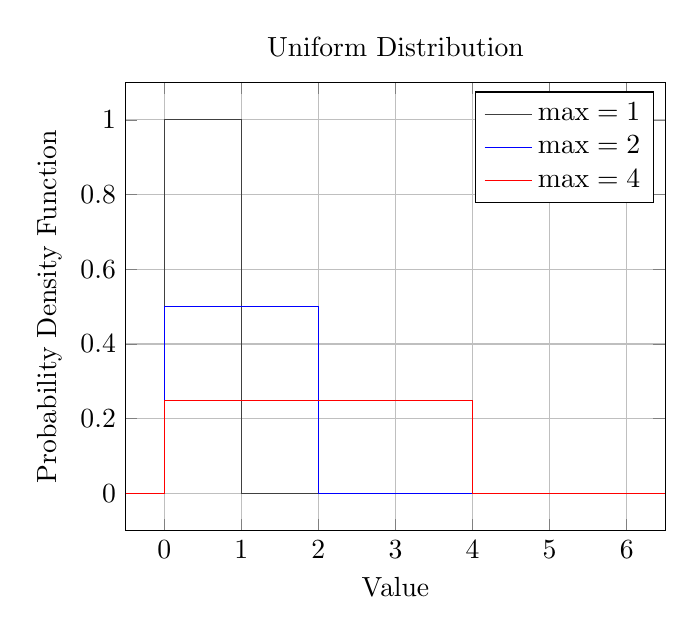
\begin{tikzpicture}
\begin{axis}[
	title={Uniform Distribution},
	xlabel={Value},
	xmin=-0.5, xmax=6.5,
	xmajorgrids,
	ylabel={Probability Density Function},
	ymajorgrids]
\addplot[darkgray] coordinates {
	(-0.5,0) (0,0) (0,1) (1,1) (1,0) (6.5,0)};
\addlegendentry{$\max = 1$}

\addplot[blue] coordinates {
	(-0.5,0) (0,0) (0,0.5) (2,0.5) (2,0) (6.5,0)};
\addlegendentry{$\max = 2$}

\addplot[red] coordinates {
	(-0.5,0) (0,0) (0,0.25) (4,0.25) (4,0) (6.5,0)};
\addlegendentry{$\max = 4$}
\end{axis}
\end{tikzpicture}
\end{center}
\caption{This figure shows the PDFs of uniform random variables with support intervals $[0,1]$, $[0,2]$ and $[0,4]$.}
\end{figure}

\begin{example}
David comes to campus every morning riding the Aggie Spirit Transit.
On his route, a bus comes every thirty minutes, from sunrise until dusk.
David, who does not believe in alarm clocks or watches, wakes up randomly.
After cooking a hefty breakfast, he walks to the bus stop.
If his arrival time at the bus stop is uniformly distributed between 9:00 a.m.\ and 9:30 a.m., what is the probability that he waits less than five minutes for the bus?

Let $t_0$ be the time at which David arrives at the bus stop, and denote by $T$ the time he spends waiting.
The time at which the next bus arrives at David's stop is uniformly distributed between $t_0$ and $t_0 + 30$.
The amount of time that he spends at the bus stop is therefore uniformly distributed between $0$ and $30$ minutes.
Accordingly, we have
\begin{equation*}
f_T(t) = \begin{cases} \frac{1}{30}, & t \in [0, 30] \\
0, & \text{otherwise}. \end{cases}
\end{equation*}
The probability that David waits less than five minutes is
\begin{equation*}
\Pr (T < 5) = \int_0^5 \frac{1}{30} dt = \frac{1}{6} .
\end{equation*}
\end{example}


\subsection{The Gaussian (Normal) Random Variable}

The \emph{Gaussian random variable} is of fundamental importance in probability and statistics. \index{Gaussian random variable}
It is often used to model distributions of quantities influenced by large numbers of small random components.
The PDF of a Gaussian random variable is given by
\begin{equation*}
f_X (x) = \frac{1}{\sqrt{2 \pi} \sigma} e^{- \frac{(x - m)^2}{2 \sigma^2}}
\quad - \infty < x < \infty,
\end{equation*}
where $m$ and $\sigma > 0$ are real parameters.

\begin{figure}[ht]
\begin{center}
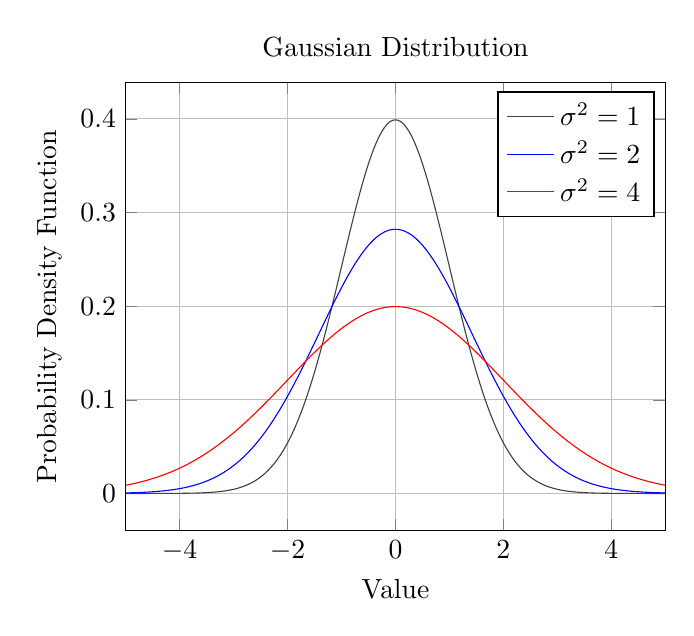
\begin{tikzpicture}
\begin{axis}[
	title={Gaussian Distribution},
	xlabel={Value},
	xmin=-5, xmax=5,
	xmajorgrids,
	ylabel={Probability Density Function},
	ymajorgrids]
\addplot[darkgray,domain=-5:5,samples=201]
	{exp(-((x^2)/2))/sqrt(2*pi)};
\addlegendentry{$\sigma^2 = 1$}

\addplot[blue,domain=-5:5,samples=201]
	{exp(-((x^2)/4))/sqrt(4*pi)};
\addlegendentry{$\sigma^2 = 2$}

\addplot[red,domain=-5:5,samples=201]
	{exp(-((x^2)/8))/sqrt(8*pi)};
\addlegendentry{$\sigma^2 = 4$}
\end{axis}
\end{tikzpicture}
\end{center}
\caption{The distributions of Gaussian random variables appear above for parameters $m = 0$ and $\sigma^2 \in \{ 1, 2, 4 \}$.}
\end{figure}

A Gaussian variable whose distribution has parameters $m = 0$ and $\sigma = 1$ is called a \emph{normal random variable} or a \emph{standard Gaussian random variable}, names that hint at its popularity. \index{Normal random variable}
The CDF of a Gaussian random variable does not admit a closed-form expression; it can be expressed as
\begin{equation*}
\begin{split}
F_X (x) &= \Pr (X \leq x)
= \frac{1}{\sqrt{2 \pi} \sigma}
\int_{- \infty}^{x} e^{- \frac{(u - m)^2}{2 \sigma^2}} du \\
&= \frac{1}{\sqrt{2 \pi}}
\int_{- \infty}^{(x - m)/\sigma} e^{- \frac{v^2}{2}} dv
= \Phi \left( \frac{x - m}{\sigma} \right),
\end{split}
\end{equation*}
where $\Phi (\cdot)$ is termed the \emph{standard normal cumulative distribution function} and is defined by
\begin{equation*}
\Phi (x) = 
\frac{1}{\sqrt{2 \pi}} \int_{-\infty}^x e^{-\frac{v^2}{2}} dv .
\end{equation*}
We emphasize that the function $\Phi (\cdot)$ is nothing more than a convenient notation for the CDF of a normal random variable.

\begin{example} \label{example:NoiseCommunicationSystem1}
A binary message is transmitted through a noisy communication channel (e.g., a long wire).
The message $X$ takes on either a value of $1$ or $-1$ with equal probability (e.g., a voltage of $\pm 1 V$ is applied to one end of the wire).
A random variable $Y$ is observed at the output of the communication channel (e.g., the measured voltage at the other end of the wire).
If the dominant impairment is additive thermal noise $Z$, then one typically models the system with $Y = X + Z$ and assumes that $Z$ is a Gaussian random variable with mean 0.
In this case, the receiver declares that a $1$ (or $-1$) was transmitted if the sent signal is positive (or negative).
What is the probability of making an erroneous decision?

Let $S \in \{ -1, 1 \}$ denote the transmitted signal, $N$ be the value of the thermal noise, and $Y$ represent the value of the received signal.
An error can occur in one of two possible ways: $S = 1$ was transmitted and $Y$ is less than zero, or $S = -1$ was transmitted and $Y$ is greater than zero.
Using the total probability theorem, we can compute the probability of error as
\begin{equation*}
\Pr (Y \geq 0 | S = -1) \Pr (S = -1)
+ \Pr (Y \leq 0 | S = 1) \Pr (S = 1).
\end{equation*}
By symmetry, it is easily argued that
\begin{equation*}
\begin{split}
\Pr (Y \leq 0 | S = 1) &= \Pr (Y \geq 0 | S = -1) = \Pr (N > 1) \\
&= \int_{1}^{\infty} \frac{1}{\sqrt{2 \pi} \sigma}
e^{- \frac{u^2}{2 \sigma^2}} du
= 1 - \Phi \left( \frac{1}{\sigma} \right) .
\end{split}
\end{equation*}
The probability that the receiver makes an erroneous decision is $1 - \Phi (1/\sigma)$.
The reliability of this transmission scheme depends on the amount of noise present at the receiver.
\end{example}

The normal random variable is so frequent in applied mathematics and engineering that many variations of its CDF possess their own names.
The \emph{error function} is a function which is primarily encountered in the fields of statistics and partial differential equations. \index{Error function}
It is defined by
\begin{equation*}
\mathrm{erf} (x) = \frac{2}{\sqrt{\pi}} \int_0^x e^{-u^2} du .
\end{equation*}
The error function is related to the standard normal cumulative distribution function by scaling and translation,
\begin{equation*}
\Phi (x) = \frac{1 + \mathrm{erf} \left( {x}/{\sqrt{2}} \right)}{2}.
\end{equation*}
If $X$ is a standard normal random variable, then $\mathrm{erf} \left( x/{\sqrt{2}} \right)$ denotes the probability that $X$ lies in the interval $(-x, x)$.
In engineering, it is customary to employ the \emph{$Q$-function}, which is given by \index{Q-function}
\begin{equation} \label{equation:Qfunction}
\begin{split}
Q (x) &= \frac{1}{\sqrt{2 \pi}} \int_x^{\infty} e^{-\frac{u^2}{2}} du
= 1 - \Phi (x) \\
&= \frac{ 1 - \mathrm{erf} \left( {x}/{\sqrt{2}} \right) }{2} .
\end{split}
\end{equation}
Equation \eqref{equation:Qfunction} may prove useful when using software packages that provide a built-in implementation for $\mathrm{erf}(\cdot)$, but not for the $Q$-function.
The probability of an erroneous decision in Example~\ref{example:NoiseCommunicationSystem1} can be expressed concisely using the Q-function as $Q (1/\sigma)$.


Next, we prove that the standard normal PDF integrates to one.
The solution is easy to follow, but hard to discover.
It is therefore useful to include it in this document.
Consider a standard normal PDF,
\begin{equation*}
f_X(x) = \frac{1}{\sqrt{2 \pi}} e^{- \frac{x^2}{2}} .
\end{equation*}
We can show that $f_X (x)$ integrates to one using a subtle argument and a change of variables.
We start with the square of the integrated PDF and proceed from there,
\begin{equation*}
\begin{split}
\left(\int_{- \infty}^{\infty} f_X (u) du \right)^2
&= \int_{- \infty}^{\infty} \frac{1}{\sqrt{2 \pi}} e^{- \frac{u^2}{2}} du
\int_{- \infty}^{\infty} \frac{1}{\sqrt{2 \pi}} e^{- \frac{v^2}{2}} dv \\
&= \int_{- \infty}^{\infty} \int_{- \infty}^{\infty}
\frac{1}{2 \pi} e^{- \frac{u^2 + v^2}{2}} du dv
= \int_{0}^{2 \pi} \frac{1}{2 \pi} d\theta
\int_{0}^{\infty} e^{- \frac{r^2}{2}} r dr \\
&= \left. \left( - e^{- \frac{r^2}{2}} \right) \right|_0^{\infty} = 1.
\end{split}
\end{equation*}
Since the square of the desired integral is nonnegative and equal to one, we can conclude that the normal PDF integrates to one.

\begin{example}
We wish to calculate the mean and variance of a Gaussian random variable with parameters $m$ and $\sigma^2$.
By definition, the PDF of this random variable can be written as
\begin{equation*}
f_X (u) = \frac{1}{\sqrt{2 \pi} \sigma} e^{-\frac{(u - m)^2}{2\sigma^2}}
\quad u \in \RealNumbers .
\end{equation*}
The mean of $X$ can be obtained through direct integration, with a change of variables,
\begin{equation*}
\begin{split}
\Expect [X]
&= \frac{1}{\sqrt{2 \pi} \sigma} \int_{- \infty}^{\infty} u e^{-\frac{(u-m)^2}{2\sigma^2}} du \\
&= \frac{\sigma}{\sqrt{2 \pi}} \int_{- \infty}^{\infty}
\left( v+\frac{m}{\sigma} \right) e^{-\frac{v^2}{2}} dv \\
&= \frac{\sigma}{\sqrt{2 \pi}} \int_{- \infty}^{\infty}
v e^{-\frac{v^2}{2}} dv
+ \frac{\sigma}{\sqrt{2 \pi}} \int_{- \infty}^{\infty}
\frac{m}{\sigma} e^{-\frac{v^2}{2}} dv
= m.
\end{split}
\end{equation*}
In finding a solution, we have leveraged the facts that $v e^{-\frac{v^2}{2}}$ is an absolutely integrable, odd function.
We also took advantage of the normalization condition which ensures that a Gaussian PDF integrates to one.
To derive the variance, we again use the normalization condition.
For a Gaussian PDF, this property implies that
\begin{equation*}
\int_{-\infty}^{\infty} e^{- \frac{(u-m)^2}{2 \sigma^2}} du
= \sqrt{2 \pi} \sigma .
\end{equation*}
Differentiating both sides of this equation with respect to $\sigma$, we get
\begin{equation*}
\int_{-\infty}^{\infty} \frac{(u-m)^2}{\sigma^3}
e^{- \frac{(u-m)^2}{2 \sigma^2}} du
= \sqrt{2 \pi} .
\end{equation*}
Rearranging the terms yields
\begin{equation*}
\int_{-\infty}^{\infty} \frac{(u-m)^2}{\sqrt{2 \pi} \sigma}
e^{- \frac{(u-m)^2}{2 \sigma^2}} du
= \sigma^2 .
\end{equation*}
Hence, $\Var[X] = \Expect \left[ (X-m)^2 \right] = \sigma^2$.
Of course, the variance can also be obtained by more conventional methods.
\end{example}

\subsection{The Exponential Distribution}
\label{section:ExponentialDistribution}

The \emph{exponential random variable} is also frequently encountered in engineering. \index{Exponential random variable}
It can be used to model the lifetime of devices and systems, and the time elapsed between specific occurrences.
An exponential random variable $X$ with parameter $\lambda > 0$ has PDF
\begin{equation*}
f_X (x) = \lambda e^{- \lambda x} \quad x \geq 0 .
\end{equation*}
For $x \geq 0$, its CDF is equal to
\begin{equation*}
F_X (x) = 1 - e^{- \lambda x} .
\end{equation*}
The parameter $\lambda$ characterizes the rate at  which events occur.

\begin{figure}[ht]
\begin{center}
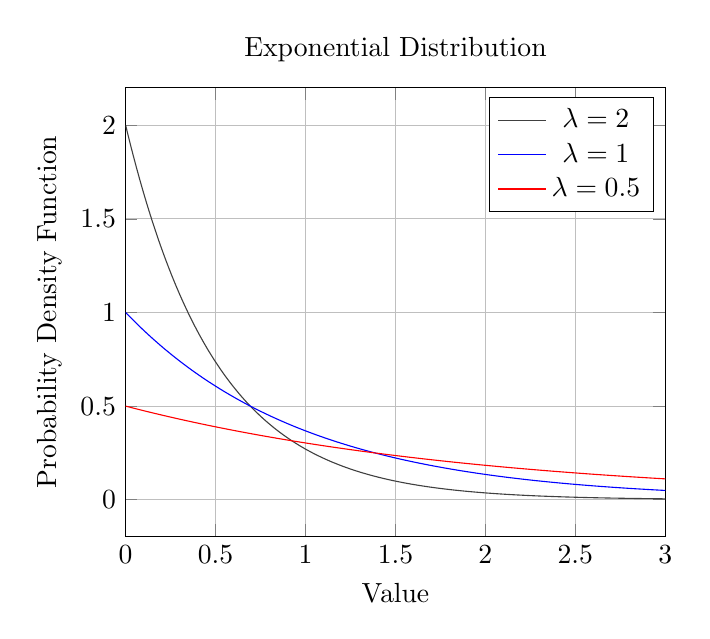
\begin{tikzpicture}
\begin{axis}[
	title={Exponential Distribution},
	xlabel={Value},
	xmin=0, xmax=3,
	xmajorgrids,
	ylabel={Probability Density Function},
	ymajorgrids]
\addplot[darkgray,domain=0:3,samples=201]
	{2*exp(-2*x)};
\addlegendentry{$\lambda = 2$}

\addplot[blue,domain=0:3,samples=201]
	{exp(-x)};
\addlegendentry{$\lambda = 1$}

\addplot[red,domain=0:3,samples=201]
	{0.5*exp(-0.5*x)};
\addlegendentry{$\lambda = 0.5$}
\end{axis}
\end{tikzpicture}
\end{center}
\caption{The distributions of exponential random variables are shown above for parameters $\lambda \in \{0.5, 1, 2 \}$.}
\end{figure}

\begin{example}
Connection requests at an Internet server are characterized by an exponential inter-arrival time with parameter $\lambda = 1/2$.
If a request arrives at time $t_0$, what is the probability that the next packet arrives within two minutes?

The probability that the inter-arrival time $T$ is less than two minutes can be computed as
\begin{equation*}
\begin{split}
\Pr ( T < 2 ) &= \int_0^2 \frac{1}{2} e^{- \frac{u}{2}} du
= \left. - e^{- \frac{u}{2}} \right|_0^2 \\
&= 1 - e^{-1} \approx 0.632 .
\end{split}
\end{equation*}
\end{example}

The exponential random variable can be obtained as the limit of a sequence of geometric random variables.
Let $\lambda$ be fixed and defined $p_n = \lambda/n$.
We define the PMF of random variable $Y_n$ as
\begin{equation*}
p_{Y_n} (k) = (1 - p_n)^{k-1} p_n
= \left( 1 - \frac{\lambda}{n} \right)^{k-1} \frac{\lambda}{n}
\quad k = 1, 2, \ldots
\end{equation*}
That is, random variable $Y_n$ is a standard geometric random variable with parameter $p_n = \lambda/n$.
For every $n$, we create a new variable $X_n$,
\begin{equation*}
X_n = \frac{Y_n}{n}.
\end{equation*}
By construction, the random variable $X_n$ has PMF
\begin{equation*}
p_{X_n} (y) = \begin{cases}
(1 - p_n)^{k-1} p_n, & y = k/n \\
0, & \text{otherwise} .
\end{cases}
\end{equation*}
For any $x \geq 0$, the CDF of random variable $X_n$ can be computed as
\begin{equation*}
\begin{split}
\Pr (X_n \leq x)
&= \Pr (Y_n \leq n x)
= \sum_{k = 1}^{\lfloor n x \rfloor} p_{Y_n} (k) \\
&= \sum_{k = 1}^{\lfloor n x \rfloor} (1 - p_n)^{k-1} p_n
% &= p_n \frac{1 - (1 - p_n)^{\lfloor n x \rfloor}}{1 - (1 - p_n)} \\
= 1 - (1 - p_n)^{\lfloor n x \rfloor} .
\end{split}
\end{equation*}
In the limit, as $n$ grows unbounded, we get
\begin{equation*}
\begin{split}
\lim_{n \rightarrow \infty} \Pr (X_n \leq x)
&= \lim_{n \rightarrow \infty} \left[ 1 - (1 - p_n)^{\lfloor n x \rfloor} \right] \\
&= 1 - \lim_{n \rightarrow \infty}
\left( 1 - \frac{\lambda}{n} \right)^{\lfloor n x \rfloor} \\
&= 1 - e^{- \lambda x} .
\end{split}
\end{equation*}
Thus, the sequence of scaled geometric random variables $\{ X_n \}$ converges in distribution to an exponential random variable $X$ with parameter $\lambda$.

\paragraph{Memoryless Property:}
In view of this asymptotic characterization and the fact that geometric random variables are memoryless, it is not surprising that the exponential random variable also satisfies the \emph{memoryless property}, \index{Memoryless property}
\begin{equation*}
\Pr (X > t + u | X > t) = \Pr (X > u).
\end{equation*}
This fact can be shown by a straightforward application of conditional probability.
Suppose that $X$ is an exponential random variable with parameter $\lambda$.
Also, let $t$ and $u$ be two positive numbers.
The memoryless property can be verified by expanding the conditional probability of $X$ using definition \eqref{equation:ConditionalProbability},
\begin{equation*}
\begin{split}
\Pr (X > t + u | X > t)
&= \frac{\Pr( \{ X > t + u \} \cap \{ X > t \} ) }{ \Pr ( X > t ) } \\
&= \frac{\Pr( X > t + u ) }{ \Pr ( X > t ) }
= \frac{e^{- \lambda (t + u)} }{ e^{- \lambda t } } \\
&= e^{- \lambda u } = \Pr (X > u).
\end{split}
\end{equation*}
In reality, the exponential random variable is the only continuous random variable that satisfies the memoryless property.

\begin{example}
A prominent company, Century Oak Networks, maintains a bank of servers for its operation.
Hard drives on the servers have a half-life of two years.
We wish to compute the probability that a specific disk needs repair within its first year of usage.

Half-lives are typically used to describe quantities that undergo exponential decay.
Let $T$ denote the time elapsed until failure of the disk.
We know that $T$ is an exponential random variable and, although we are not given $\lambda$ explicitly, we know that
\begin{equation*}
\Pr ( T > 2 ) = \frac{1}{2} .
\end{equation*}
We use the memoryless property to solve this problem,
\begin{equation*}
\begin{split}
\Pr (T > 2) &= \Pr (T > 1) \Pr (T > 1 + 1 | T > 1) \\
&= \Pr (T > 1) \Pr (T > 1)
= \left( \Pr(T > 1) \right)^2 .
\end{split}
\end{equation*}
It follows that $\Pr (T > 1) = \sqrt{ \Pr (T > 2) } = 1 / \sqrt{2}$.
We can then write $\Pr (T < 1) = 1 - \Pr (T > 1) \approx 0.293$.
An alternative way to solve this problem would be to first find the value of $\lambda$ associated with $T$, and then compute $\Pr (T < 1)$ from the corresponding integral.
\end{example}


\section{Additional Distributions}

Probability distributions arise in many different contexts and they assume various forms.
We conclude this first chapter on continuous random variables by mentioning a few additional distributions that find application in engineering.
It is interesting to note the interconnection between various random variables and their corresponding probability distributions.


\subsection{The Gamma Distribution}

The gamma PDF defines a versatile collection of distributions.
The PDF of a \emph{gamma random variable} is given by \index{Gamma random variable}
\begin{equation*}
f_X (x) = \frac{\lambda (\lambda x)^{\alpha - 1} e^{-\lambda x}}{\Gamma (\alpha)} \quad  x > 0,
\end{equation*}
where $\Gamma(\cdot)$ denotes the gamma function defined by
\begin{equation*}
\Gamma (z) = \int_0^{\infty} u^{z-1} e^{-u} du \quad z > 0 .
\end{equation*}
The two parameters $\alpha > 0$ and $\lambda > 0$ affect the shape of the ensuing distribution significantly.
By varying these two parameters, it is possible for the gamma PDF to accurately model a wide array of empirical data.

The gamma function can be evaluated recursively using integration by parts; this yields the relation $\Gamma (z+1) = z \Gamma (z)$ for $z > 0$.
For nonnegative integers, it can easily be shown that $\Gamma (k + 1) = k!$.
Perhaps, the most well-known value for the gamma function at a non-integer argument is $\Gamma ( 1/2 ) = \sqrt{\pi}$.
Interestingly, this specific value for the gamma function can be evaluated by a procedure similar to the one we used to integrate the Gaussian distribution,
\begin{equation*}
\begin{split}
\left( \Gamma \left( \frac{1}{2} \right) \right)^2
&= \int_0^{\infty} u^{-\frac{1}{2}} e^{-u} du
\int_0^{\infty} v^{-\frac{1}{2}} e^{-v} dv \\
&= \int_0^{\infty} \int_0^{\infty}
u^{-\frac{1}{2}} v^{-\frac{1}{2}} e^{-(u + v)}
du dv \\
&= \int_0^{\pi / 2} \int_0^{\infty}
\frac{1}{r^2 \sin \theta \cos \theta} e^{-r^2}
4 r^3 \sin \theta \cos \theta dr d\theta \\
&= \int_0^{\pi / 2} \int_0^{\infty}
 e^{-r^2} 4 r dr d\theta
= \pi .
\end{split}
\end{equation*}
Many common distributions are special cases of the gamma distribution, as seen in Figure~\ref{figure:GammaDistribution}.

\begin{figure}[ht]
\begin{center}
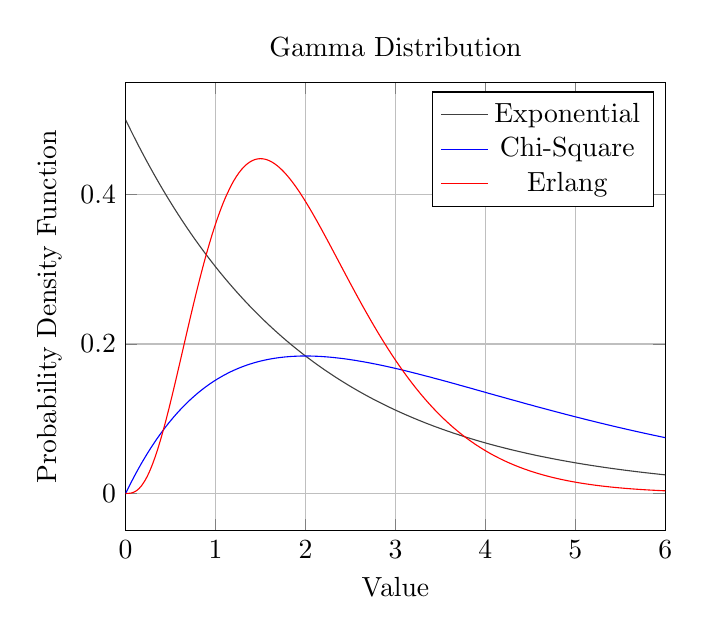
\begin{tikzpicture}
\begin{axis}[
	title={Gamma Distribution},
	xlabel={Value},
	xmin=0, xmax=6,
	xmajorgrids,
	ylabel={Probability Density Function},
	ymajorgrids]
\addplot[darkgray,domain=0:6,samples=201]
	{0.5*exp(-0.5*x)};
\addlegendentry{Exponential}

\addplot[blue,domain=0:6,samples=201]
	{0.25*x*exp(-0.5*x)};
\addlegendentry{Chi-Square}

\addplot[red,domain=0:6,samples=201]
	{(8/3)*(x^3)*exp(-2*x)};
\addlegendentry{Erlang}
\end{axis}
\end{tikzpicture}
\end{center}
\caption{Gamma distributions form a two-parameter family of PDFs and, depending on $(\alpha, \lambda)$, they can be employed to model various situations.
The parameters used above are $(1, 0.5)$ for the exponential distribution, $(2, 0.5)$ for the chi-square distribution and $(4, 2)$ for the Erlang distribution;
they are all instances of gamma distributions.}
\label{figure:GammaDistribution}
\end{figure}

\paragraph{The Exponential Distribution:}
When $\alpha = 1$, the gamma distribution simply reduces to the exponential distribution discussed in Section~\ref{section:ExponentialDistribution}.

\paragraph{The Chi-Square Distribution:}
When $\lambda = 1/2$ and $\alpha = k/2$ for some positive integer $k$, the gamma distribution becomes a \emph{chi-square distribution},
\begin{equation*}
f_X (x) = \frac{x^{\frac{k}{2} - 1} e^{-\frac{x}{2}}}{2^{\frac{k}{2}}\Gamma (k/2)} \quad  x > 0.
\end{equation*}
The chi-square distribution is one of the probability distributions most widely used in statistical inference problems.
Interestingly, the sum of the squares of $k$ independent standard normal random variables leads to a chi-square variable with $k$ degrees of freedom.


\paragraph{The Erlang Distribution:}
When $\alpha = m$, a positive integer, the gamma distribution is called an \emph{Erlang distribution}.
This distribution finds application in queueing theory.
Its PDF is given by
\begin{equation*}
f_X (x) = \frac{\lambda (\lambda x)^{m - 1} e^{-\lambda x}}{(m-1)!} \quad  x > 0.
\end{equation*}
An $m$-Erlang random variable can be obtained by summing $m$ independent exponential random variables.
Specifically, let $X_1, X_2, \ldots, X_m$ be independent exponential random variables, each with parameter $\lambda > 0$.
The random variable $S_m$ given by
\begin{equation*}
S_m = \sum_{k=1}^m X_k
\end{equation*}
is an Erlang random variable with parameter $m$ and $\lambda$.

\begin{example}
Suppose that the requests arriving at a computer server on the Internet are characterized by independent, memoryless inter-arrival periods.
Let $S_m$ be a random variable that denotes the time instant of the $m$th arrival, then $S_m$ is an Erlang  random variable.
\end{example}


\subsection{The Rayleigh Distribution}

The Rayleigh PDF is given by \index{Rayleigh random variable}
\begin{equation*}
f_R (r) = \frac{r}{\sigma^2} e^{- \frac{r^2}{2 \sigma^2} } \quad r \geq 0 .
\end{equation*}
The \emph{Rayleigh distribution} arises in the context of wireless communications.
Suppose that $X$ and $Y$ are two independent normal random variables, then the magnitude of this random vector possesses a Rayleigh distribution.
Also, if $R$ is a Rayleigh random variable then $R^2$ has an exponential distribution.

\begin{figure}[ht]
\begin{center}
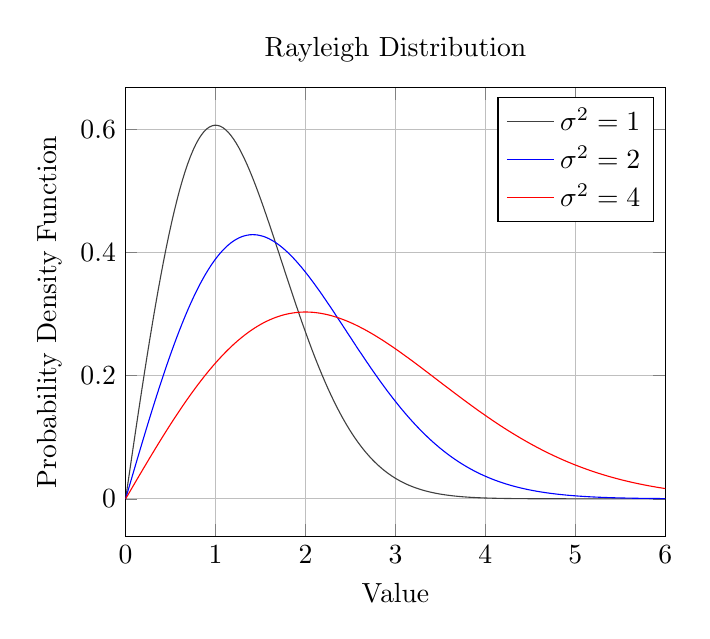
\begin{tikzpicture}
\begin{axis}[
	title={Rayleigh Distribution},
	xlabel={Value},
	xmin=0, xmax=6,
	xmajorgrids,
	ylabel={Probability Density Function},
	ymajorgrids]
\addplot[darkgray,domain=0:6,samples=201]
	{x*exp(-0.5*(x^2))};
\addlegendentry{$\sigma^2 = 1$}

\addplot[blue,domain=0:6,samples=201]
	{0.5*x*exp(-0.25*(x^2))};
\addlegendentry{$\sigma^2 = 2$}

\addplot[red,domain=0:6,samples=201]
	{0.25*x*exp(-0.125*(x^2))};
\addlegendentry{$\sigma^2 = 4$}
\end{axis}
\end{tikzpicture}
\end{center}
\caption{This figure plots the distributions of Rayleigh random variables for parameters $\sigma^2 \in \{ 1, 2, 4 \}$.}
\end{figure}

\begin{example}
Radio signals propagating through wireless media get reflected, refracted and diffracted.
This creates variations in signal strength at the destinations, a phenomenon known as fading.
Rayleigh random variables are often employed to model amplitude fluctuations of radio signals in urban environments.
\end{example}

\begin{example}
Suppose that $R$ is a Rayleigh random variable with parameter $\sigma^2$.
We wish to compute its mean and variance.

Recall that $R$ is a nonnegative random variable with PDF
\begin{equation*}
f_R (r) = \frac{r}{\sigma^2} e^{- \frac{r^2}{2 \sigma^2} } \quad r \geq 0 .
\end{equation*}
Using this distribution, we get
\begin{equation*}
\begin{split}
\Expect [R] &= \int_0^{\infty} u f_R(u) du
= \int_0^{\infty} \frac{u^2}{\sigma^2} e^{- \frac{u^2}{2 \sigma^2}} du \\
&= \left. - u e^{- \frac{u^2}{2 \sigma^2}} \right|_0^{\infty}
+ \int_0^{\infty} e^{- \frac{u^2}{2 \sigma^2}} du \\
&= \sqrt{ 2 \pi } \sigma
\int_0^{\infty} \frac{1}{\sqrt{2 \pi} \sigma} e^{- \frac{v^2}{2 \sigma^2}} dv
= \frac{\sqrt{2 \pi} \sigma}{2} .
\end{split}
\end{equation*}
Integration by parts is key in solving this expectation.
Also, notice the judicious use of the fact that the integral of a standard normal random variable over $[0, \infty)$ must be equal to $1/2$.
We compute the second moment of $R$ below,
\begin{equation*}
\begin{split}
\Expect \left[ R^2 \right] &= \int_0^{\infty} u^2 f_R(u) du
= \int_0^{\infty} \frac{u^3}{\sigma^2} e^{- \frac{u^2}{2 \sigma^2}} du \\
&= \left. - u^2 e^{- \frac{u^2}{2 \sigma^2}} \right|_0^{\infty}
+ \int_0^{\infty} 2 u e^{- \frac{u^2}{2 \sigma^2}} du \\
&= \left. - 2 \sigma^2 e^{- \frac{u^2}{2 \sigma^2}} \right|_0^{\infty}
= 2 \sigma^2 .
\end{split}
\end{equation*}
The variance of $R$ is therefore equal to
\begin{equation*}
\Var [R] = \frac{(4 - \pi)}{2} \sigma^2 .
\end{equation*}
Typically, $\sigma^2$ is employed to denote the variance of a random variable.
It may be confusing at first to have a random variable $R$ described in terms of parameter $\sigma^2$ whose variance is equal to $(4 - \pi) \sigma^2/2$.
This situation is an artifact of the following relation.
A Rayleigh random variable $R$ can be generated through the expression $R = \sqrt{X^2 + Y^2}$, where $X$ and $Y$ are independent zero-mean Gaussian variables with variance $\sigma^2$.
Thus, the parameter $\sigma^2$ in $f_R (\cdot)$ is a tribute to this popular construction, not a representation of its actual variance.
\end{example}


\subsection{The Laplace Distribution}

The \emph{Laplace distribution} is sometimes called a double exponential distribution because it can be thought of as an exponential function and its reflection spliced together. \index{Laplace random variable}
The PDF of a Laplacian random variable can then be written as
\begin{equation*}
f_X (x) = \frac{1}{2b} e^{- \frac{|x|}{b}} \quad x \in \RealNumbers ,
\end{equation*}
where $b$ is a positive constant.
The difference between two independent and identically distributed exponential random variables is governed by a Laplace distribution.

\begin{figure}[ht]
\begin{center}
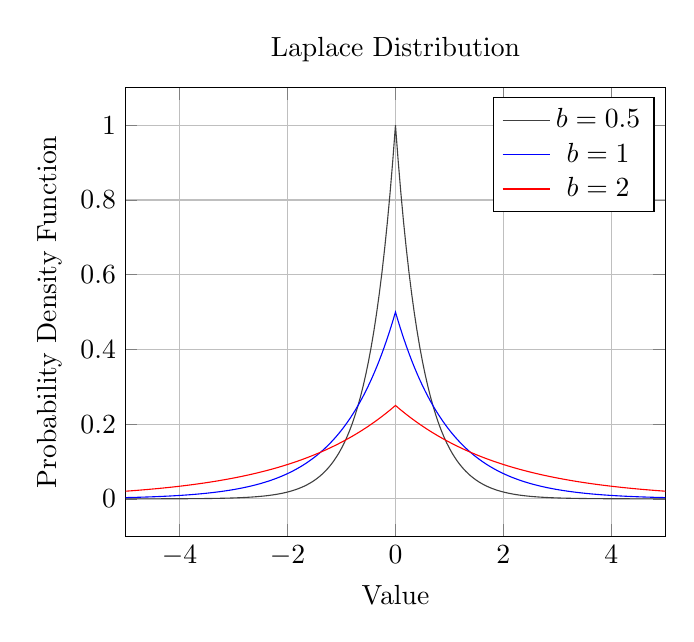
\begin{tikzpicture}
\begin{axis}[
	title={Laplace Distribution},
	xlabel={Value},
	xmin=-5, xmax=5,
	xmajorgrids,
	ylabel={Probability Density Function},
	ymajorgrids]
\addplot[darkgray,domain=-5:5,samples=201]
	{exp(-2*abs(x))};
\addlegendentry{$b = 0.5$}

\addplot[blue,domain=-5:5,samples=201]
	{0.5*exp(-abs(x))};
\addlegendentry{$b = 1$}

\addplot[red,domain=-5:5,samples=201]
	{0.25*exp(-0.5*abs(x))};
\addlegendentry{$b = 2$}
\end{axis}
\end{tikzpicture}
\end{center}
\caption{The PDF of a Laplace random variable can be constructed using an exponential function and its reflection spliced together.
This figure shows Laplace PDFs for parameters $b \in \{0.5, 1, 2 \}$.}
\end{figure}


\subsection{The Cauchy Distribution}

The \emph{Cauchy distribution} is considered a heavy-tail distribution because its tail is not exponentially bounded. \index{Cauchy random variable}
The PDF of a Cauchy random variable is given by
\begin{equation*}
f_X (x) = \frac{ \gamma }{\pi \left( \gamma^2 + x^2 \right)} \quad x \in \RealNumbers .
\end{equation*}
An interesting fact about this distribution is that its mean, variance and all higher moments are undefined.
Moreover, if $X_1, X_2, \ldots, X_n$ are independent random variables, each with a standard Cauchy distribution, then the sample mean $(X_1 + X_2 + \cdots + X_n)/n$ possesses the same Cauchy distribution.
Cauchy random variables appear in detection theory to model communication systems subject to extreme noise conditions; they also finds applications in physics.
Physicists sometimes refer to this distribution as the \emph{Lorentz distribution}.

\begin{figure}[ht]
\begin{center}
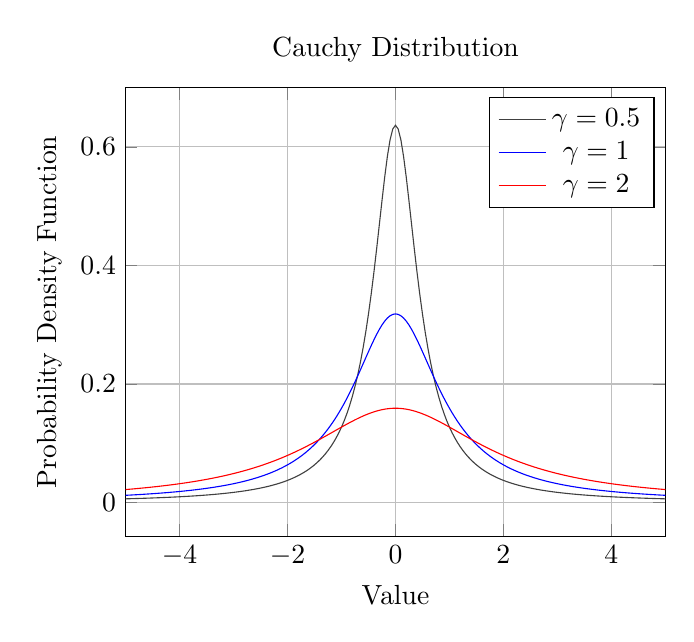
\begin{tikzpicture}
\begin{axis}[
	title={Cauchy Distribution},
	xlabel={Value},
	xmin=-5, xmax=5,
	xmajorgrids,
	ylabel={Probability Density Function},
	ymajorgrids]
\addplot[darkgray,domain=-5:5,samples=201]
	{0.5 / (pi * (0.25 + x^2)};
\addlegendentry{$\gamma = 0.5$}

\addplot[blue,domain=-5:5,samples=201]
	{1 / (pi * (1 + x^2)};
\addlegendentry{$\gamma = 1$}

\addplot[red,domain=-5:5,samples=201]
	{2 / (pi * (4 + x^2)};
\addlegendentry{$\gamma = 2$}
\end{axis}
\end{tikzpicture}
\end{center}
\caption{Cauchy distributions are categorized as heavy-tail distributions because of their very slow decay.
The PDFs of Cauchy random variables are plotted above for parameters $\gamma \in \{ 0.5, 1, 2 \}$.}
\end{figure}


\section*{Further Reading}

\begin{small}
\begin{enumerate}
\item Ross, S., \emph{A First Course in Probability}, 7th edition, Pearson Prentice Hall, 2006: Sections~5.1, 5.3--5.6.
\item Bertsekas, D. P., and Tsitsiklis, J. N., \emph{Introduction to Probability}, Athena Scientific, 2002: Sections~3.1--3.3.
\item Gubner, J. A., \emph{Probability and Random Processes for Electrical and Computer Engineers}, Cambridge, 2006: Sections~4.1, 5.1.
\item Miller, S. L., and Childers, D. G., \emph{Probability and Random Processes with Applications to Signal Processing and Communications}, 2004: Sections~3.1--3.4.
\end{enumerate}
\end{small}

